
\chapter{Einleitung}
    \section{Motivation}
    Schach ist ein traditionsreiches und abwechslungsreiches Brettspiel, dessen Ursprung nicht genau bestimmt werden kann. Allerdings wird vermutet, dass das erste schachähnliche Spiel  \textit{Tschaturanga} seinen Ursprung in Nordindien um 600 n. Chr. hatte \cite{schachgeschichte}. Bis heute bleibt Schach ein beliebtes Spiel, das 2020 durch die Netflix Serie \textit{Damengambit} und 2022 durch den Betrugsvorwurf von Magnus Carlsen an seinen 19-jährigen Gegner Hans Niemann\footnote{Quelle: \url{https://www.sportschau.de/schach/magnus-carlsen-hans-niemann-ermittlungen-100.html} am 22. April 2023} eine größere Aufmerksamkeit erhielt (siehe Abbildung \ref{fig:Schachinteresse}). 
    
    \begin{figure}[ht]
\raggedleft
  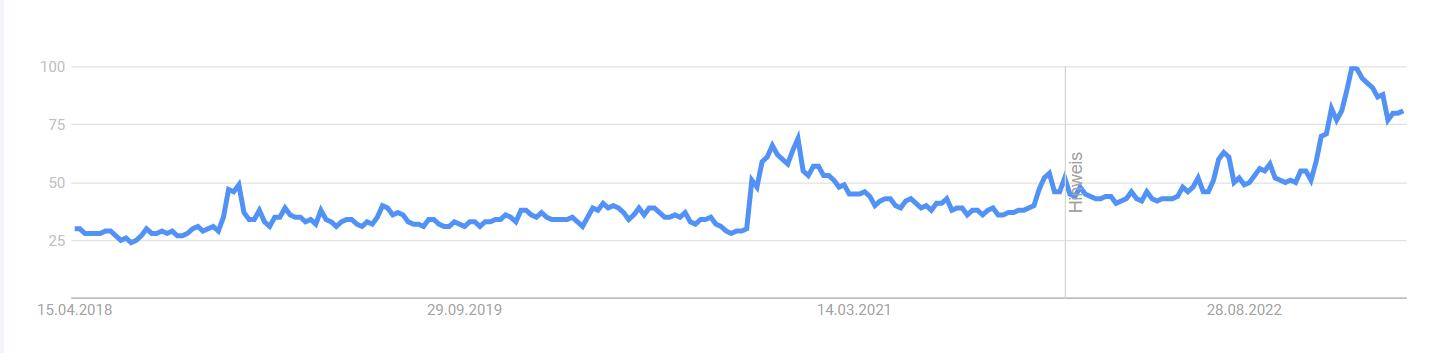
\includegraphics[width=\textwidth]{Schachentwicklung.jpg}
    \footnotesize\sffamily\textbf{Quelle:} \url{https://trends.google.de/}
  \caption{Relatives Suchinteresse des Wortes \textit{Chess} auf Google in den letzten 5 Jahren.}
  \label{fig:Schachinteresse}
\end{figure}

     Darüber hinaus hat Schach im digitalen Zeitalter eine neue Popularität erreicht. Online-Schachplattformen wie \url{chess.com} verzeichnen über zehn Millionen Schachpartien täglich\footnote{Quelle: \url{https://www.chess.com/about} am 12. Mai 2023}, während Schach Live-Streams auf Plattformen wie \url{twitch.com} Millionen von Followern anziehen\footnote{Quelle: \url{https://www.twitch.tv/chess} am 27. April 2023}.
     
Die Entwicklung einer webbasierten Multiplayer-Schach-App bietet eine einzigartige Gelegenheit, ein traditionsreiches und beliebtes Spiel im digitalen Zeitalter weiterzuentwickeln. Mein Ziel für diese Arbeit besteht darin, eine App zu entwickeln, die die Grundlagen einer Schach-App enthält und gleichzeitig eine solide Basis für zukünftige Erweiterungen und Verbesserungen bietet.
Insbesondere die Aussicht in Zukunft, innovative Funktionen zu integrieren, die bislang in den gängigen Schach-Apps nicht oder nicht kostenfrei vorhanden sind motiviert diese Arbeit. Durch die Entwicklung einer Schach-App mit neuen Funktionalitäten kann ich dazu beitragen, die Popularität von Schach zu steigern und vor allem das Spiel einem breiteren Publikum zugänglich zu machen.
    \section{Zielsetzung}
    Diese Bachelorarbeit hat das Ziel eine Schach-App zu entwerfen und zu implementieren, die eine intuitive User Experience und ein ansprechendes User Interface mit vielen nützlichen Funktionen beinhaltet. Bei der Anwendung soll dabei vor allem soziale Interaktionen im Zusammenhang mit Schach im Vordergrund stehen.
    
User Experience (kurz UX) bezieht sich darauf wie ein Nutzer sich auf einer Anwendung bewegt und wie einfach und angenehm es für den Nutzer ist, die Funktionen der Anwendung zu verwenden.
    
    Unter User Interface (kurz UI) versteht man die visuelle und interaktive Gestaltung von Benutzeroberflächen. Es umfasst die Gestaltung von Buttons, Formularen und anderen visuellen Komponenten, sowie das Feedback dieser Komponenten, wie zum Beispiel die Rückmeldung einer fehlgeschlagenen Anmeldung.
    Zusammengefasst beschäftigt sich UX damit, wie man eine Anwendung verwendet und UI damit, wie die Benutzeroberfläche der Anwendung aussieht.\cite{webdesign}
        
        Funktionen der Schach-App sind unter anderem das Registrieren und Anmelden, das Versenden, Annehmen und Ablehnen von Freundschaftsanfragen, das Zuschauen bei laufenden Spielen, das Herausfordern von Freunden zu Schachspielen und natürlich das Spielen von Schachpartien mit einem Chat und verschiedenen Einstellungsmöglichkeiten der Schachuhren selbst.
    Dabei wird besonderer Wert auf die Verwendung moderner Web-Technologien wie React, Node.js, Socket.IO, Redis und PostgeSQL gelegt, um eine optimale Benutzererfahrung und Skalierbarkeit zu gewährleisten. Darüber hinaus soll die Arbeit einen Überblick über die technischen Herausforderungen und Lösungen im Zusammenhang mit der Implementierung einer solchen Schach-App bieten.
    
Die Anwendung dient hauptsächlich als Basis Schach-App für Erweiterungen. So ist das Design noch nicht responsiv, da mit neuen Erweiterungen die UI und UX ohnehin angepasst werden muss, um alle Funktionen zur Verfügung zu stellen.
    
    \section{Aufbau der Arbeit}
Diese Bachelorarbeit gliedert sich in sechs Hauptkapitel, die jeweils unterschiedliche Aspekte der Entwicklung und Implementierung der Schach-App behandeln.

Im ersten Kapitel, der \textit{Einleitung}, werden die Motivation für die Entwicklung der Schach-App, die Zielsetzung der Arbeit und der Aufbau der Arbeit selbst vorgestellt.

Das zweite Kapitel, \textit{Theoretische Grundlagen}, erläutert die Grundlagen von Schach als Spiel sowie die verwendeten Web-Technologien wie Node.js, Express, Socket.io, React und PostgreSQL, die für das Verständnis der nachfolgenden Kapitel wichtig sind.

Im dritten Kapitel, \textit{Systemarchitektur}, wird die Gesamtarchitektur der Schach-App beschrieben, einschließlich der Unterteilung in Frontend und Backend, der Datenbankstruktur und der Kommunikation zwischen den verschiedenen Komponenten.

Das vierte Kapitel, \textit{Implementierung}, geht auf die praktische Umsetzung der Schach-App ein, indem es die Entwicklungsprozesse für das Frontend und das Backend sowie die Integration der Datenbanken erläutert.

Das fünfte Kapitel, \textit{Tests und Evaluation}, behandelt die verschiedenen Tests, die durchgeführt wurden, um die Funktionalität, Usability, Performance und Sicherheit der Schach-App zu bewerten.

Im abschließenden sechsten Kapitel, \textit{Fazit und Ausblick}, werden die Ergebnisse der Arbeit zusammengefasst, eventuelle Limitationen diskutiert und mögliche Erweiterungen und Weiterentwicklungen für die Schach-App vorgeschlagen.

Die Arbeit endet mit dem \textit{Anhang}, der zusätzliche Grafiken und die Liste der verwendeten Literatur enthält.

\section{Verwandte Arbeiten}
Es gibt vor allem zwei große online Schachplattformen: \url{chess.com} und \url{lichess.org}.

Dabei war \url{chess.com} auf Platz 114 und \url{lichess.org} auf Platz 209 der Webseiten mit am meisten Web-Traffic weltweit im April 2023\footnote{Quelle: \url{https://www.similarweb.com/website/chess.com/vs/lichess.org/#overview} am 12. Mai 2023}.

\subsection{Chess.com}
Chess.com zeichnet sich durch vielfältige Funktionen, einer verspielten UI und sehr vielen Benutzern aus. Was im Vergleich zu Lichess jedoch schnell bemerkbar ist, ist die Kommerzialisierung.

Chess.com hat auf seiner gesamten Seite viel Werbung und bietet Funktionen wie unbegrenzte Analysen der Spiele oder mehrere Partien gleichzeitig zu spielen nur bei einem monatlichen Abonnement gegen Geld an (siehe Abbildung \ref{fig:chess.com-abo}).

  \begin{figure}[htb]
  \centering
  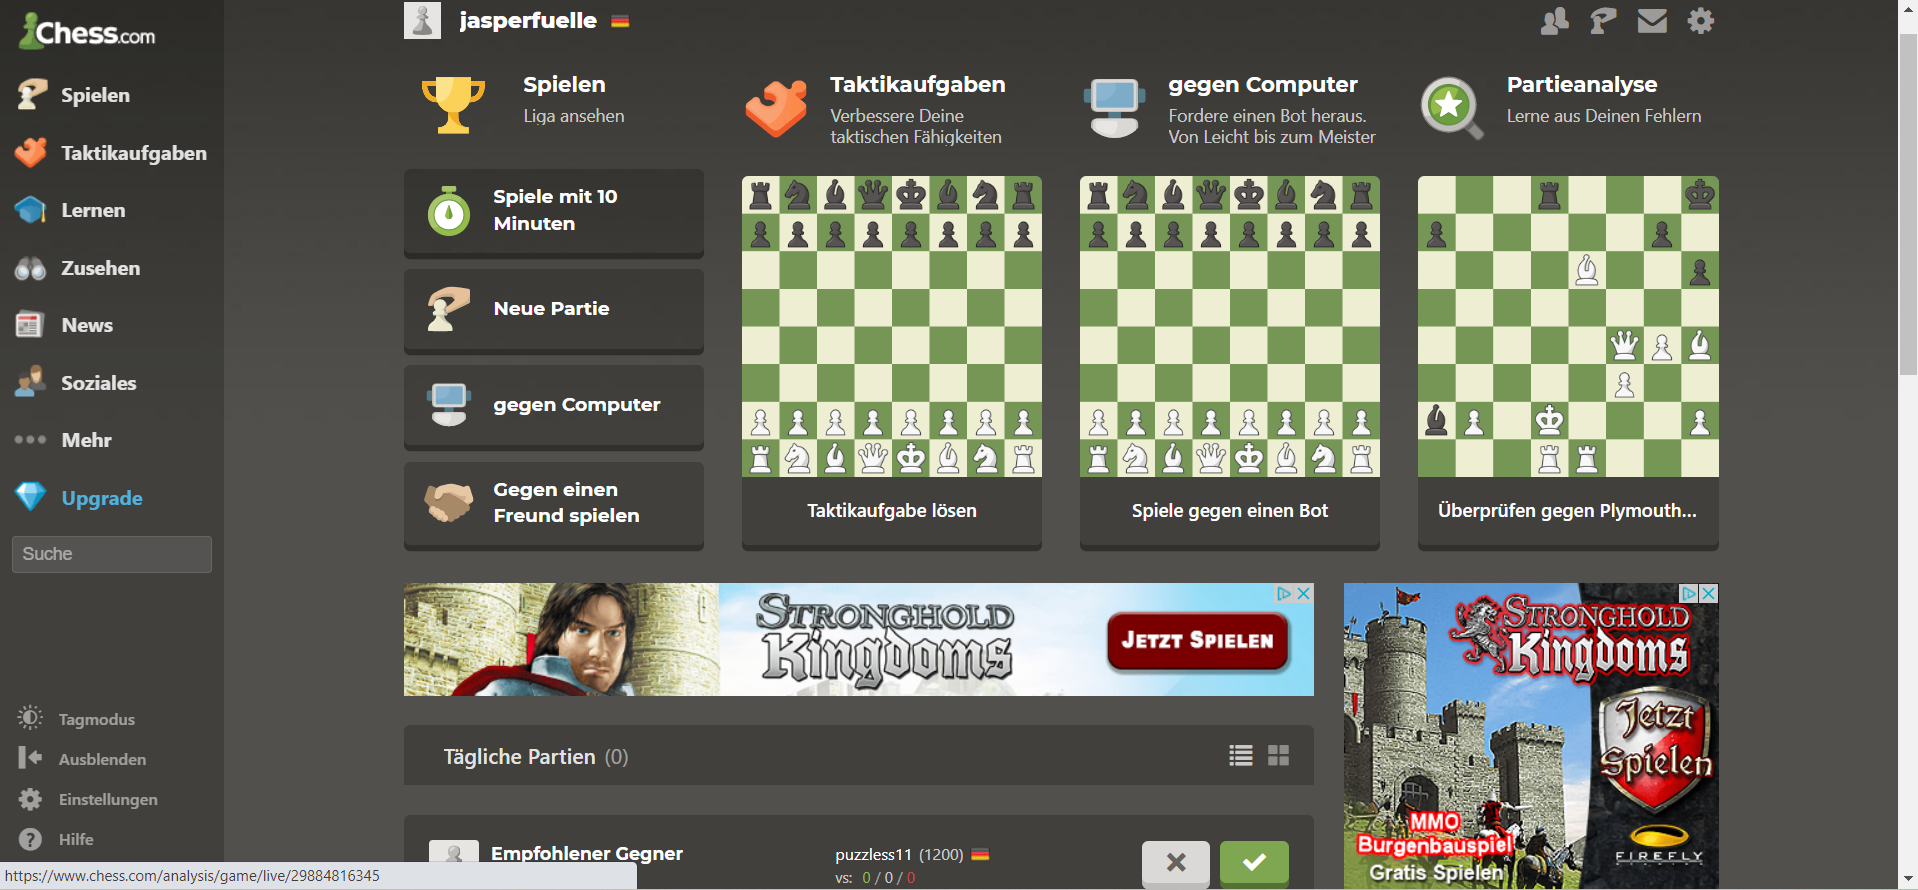
\includegraphics[width=\textwidth]{chess.com.png}
\raggedleft
    \footnotesize\sffamily\textbf{Quelle:} \url{https://www.chess.com/home} am 12. Mai 2023
  \caption{Home-Bildschirm von Chess.com}
  \label{fig:chess.com}
\end{figure}

  \begin{figure}[htb]
  \centering
  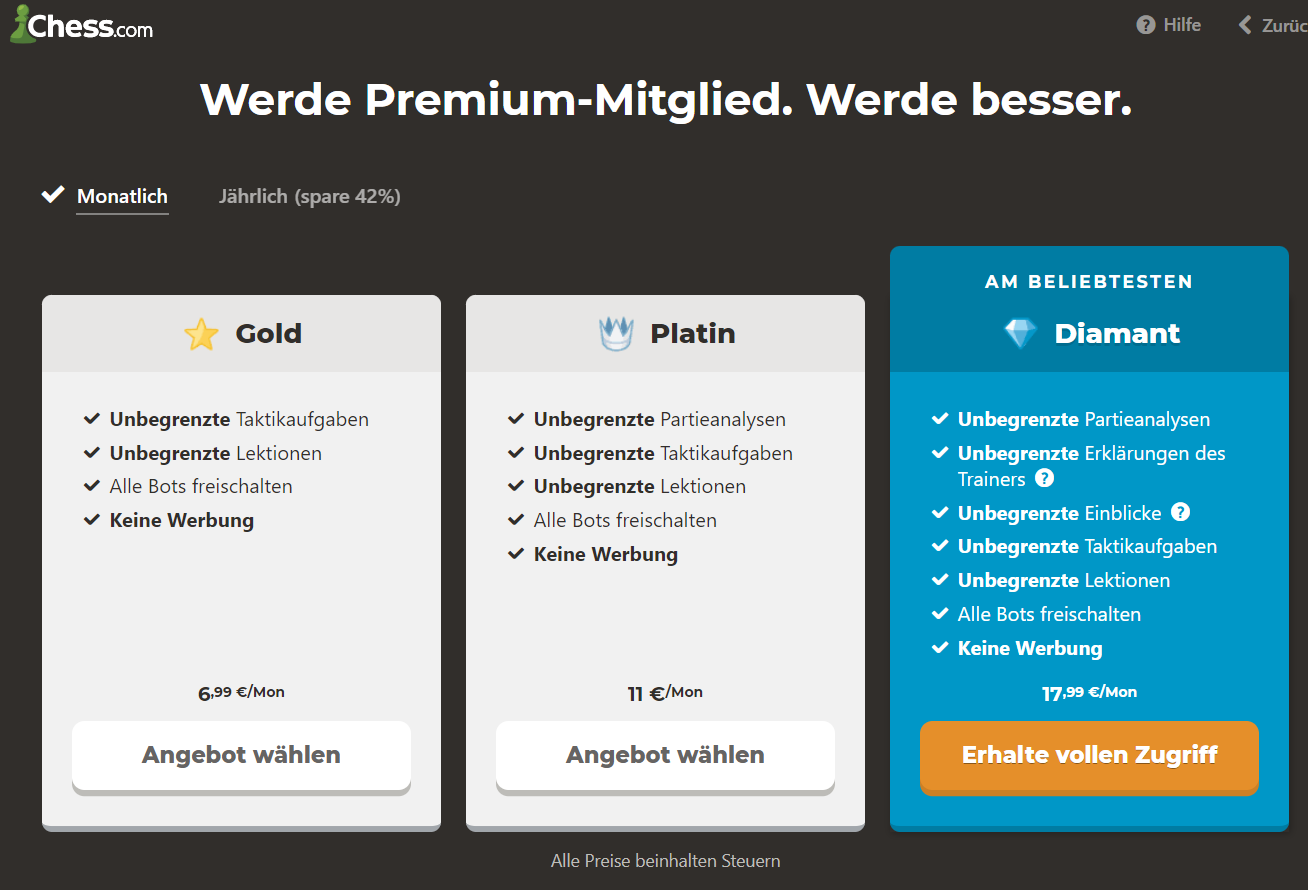
\includegraphics[width=0.7\textwidth]{Abo-chess.com.png}
  
\raggedleft

    \footnotesize\sffamily\textbf{Quelle:} \url{https://www.chess.com/membership?c=navbar} am 12. Mai 2023
  \caption{Abonnement Möglichkeiten von Chess.com}
  \label{fig:chess.com-abo}
\end{figure}

Die Funktionen die Chess.com zur Verfügung stellt (kostenpflichtige, als auch kostenfreie) sind sehr umfangreich. Es gibt Clubs mit Turnieren, es gibt viele Lektionen zum Lernen von Schach und verschiedene Spielmodi, die beispielsweise ermöglichen zu viert ein Schachspiel zu spielen.

Chess.com zeichnet sich auch durch seine Online-Präsenz auf Plattformen wie YouTube\footnote{Quelle: \url{https://www.youtube.com/@chess} am 12. Mai 2023} oder twitch\footnote{Quelle: \url{https://www.twitch.tv/chess} am 12. Mai 2023} aus.


\subsection{Lichess}
Lichess wirbt vor allem damit, dass es komplett kostenfrei verwendbar ist, keine Werbung hat und keine Registrierung nötig ist um zu spielen. Auch Funktionen wie Analysen eines Spiels sind für alle Benutzer uneingeschränkt verfügbar. Die Finanzierung von \url{lichess.org} basiert auf Spenden und die Entwicklung übernehmen Freiwillige\footnote{Quelle: \url{https://lichess.org/about} am 12. Mai 2023}. Der gesamte Code ist Open-Source und für jeden einsehbar.

Über die UI und UX von Lichess kann gestritten werden (siehe Abbildung \ref{fig:lichess}). Es ist ziemlich dunkel gehalten und einige Funktionen sind auf dem Desktop schwer zu erreichen, während sie auf einem Mobil-Gerät in der App gar nicht verfügbar sind. Dazu zählen auch soziale Interaktionen wie Gruppen. Sie sind wenig ausgebaut und schwer, bis gar nicht, zu erreichen.

  \begin{figure}[htb]
  \centering
  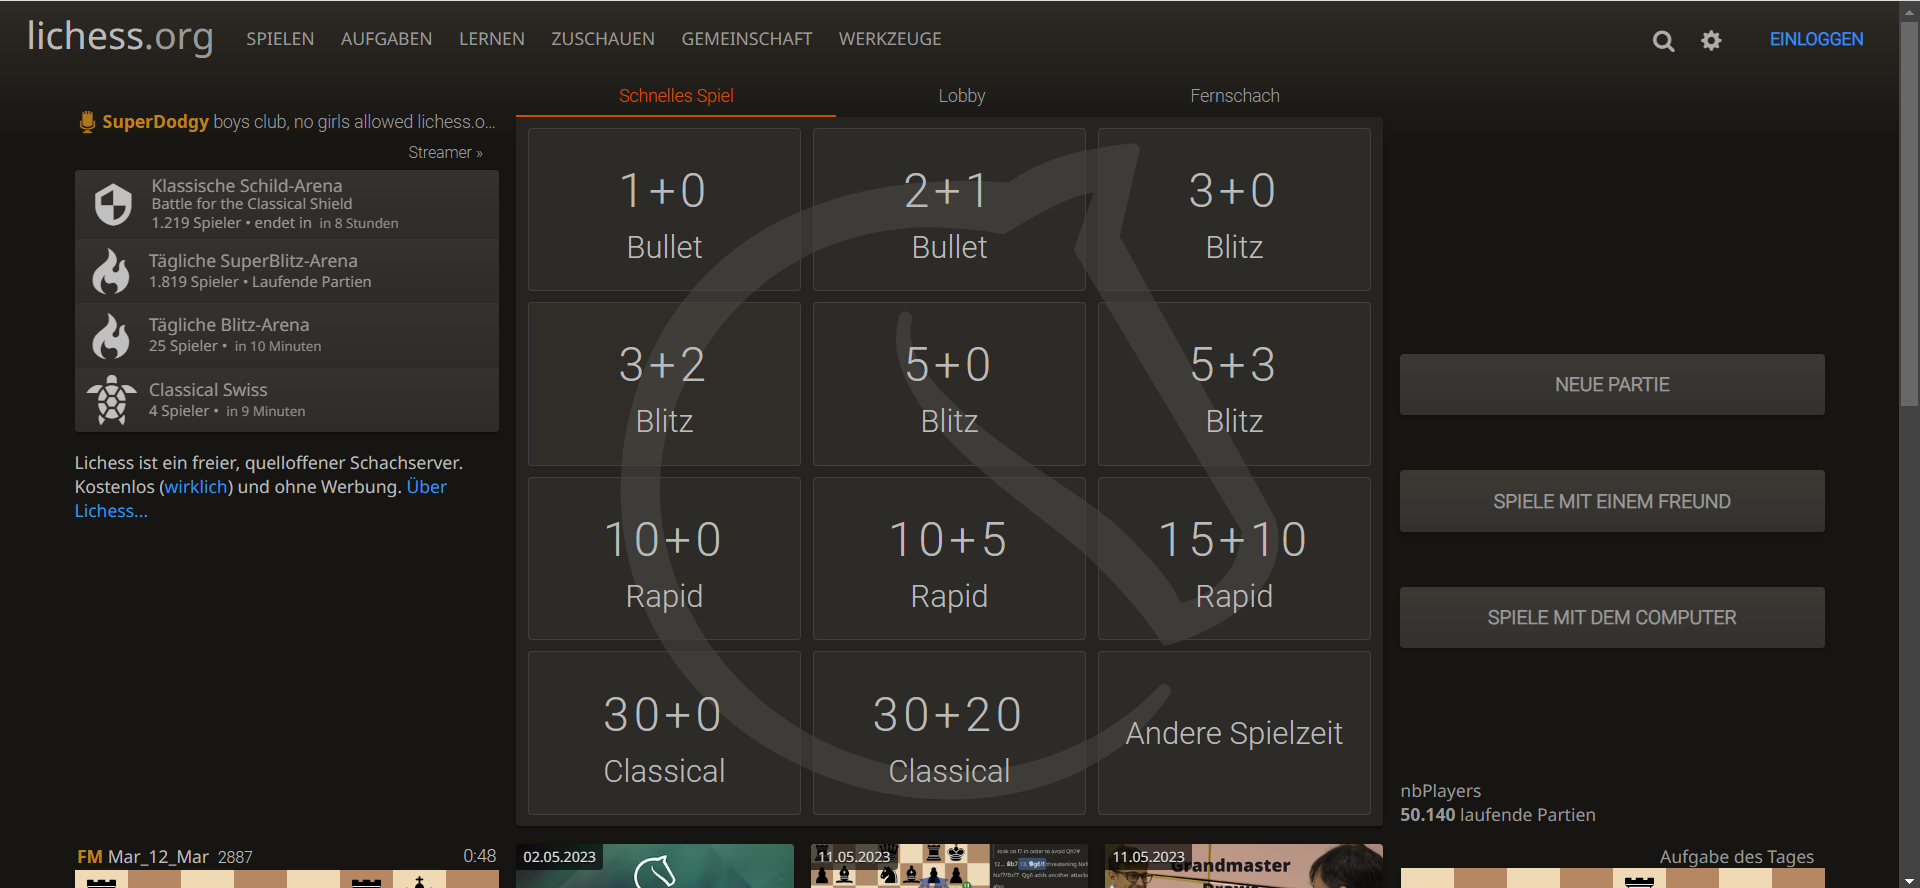
\includegraphics[width=\textwidth]{lichess.png}
\raggedleft
    \footnotesize\sffamily\textbf{Quelle:} \url{lichess.org} am 12. Mai 2023
  \caption{Der Lichess Desktop Home-Bildschirm}
  \label{fig:lichess}
\end{figure}